\documentclass[tikz]{standalone}

\usepackage{amsmath} % for \text
\usepackage{xfrac} % for \myfrac
\usepackage{bm} % for \bm
\usetikzlibrary{calc}
\usetikzlibrary{positioning}
\usetikzlibrary{decorations.pathreplacing,decorations.markings}
\usetikzlibrary{patterns} % 加载 patterns 库
\usepackage{comment}


\colorlet{myred}{red!80!black}
\colorlet{myblue}{blue!80!black}
\colorlet{mygreen}{green!60!black}
\colorlet{myorange}{orange!70!red!60!black}
\colorlet{mydarkred}{red!30!black}
\colorlet{mydarkblue}{blue!40!black}
\colorlet{mydarkgreen}{green!30!black}
\colorlet{myred2}{red!50!white}

\colorlet{mylightblue}{blue!60!cyan!80!black!15}
\colorlet{mypurple}{blue!50!red!70}
\colorlet{gaugecol}{red!90!black!70} % Wiki red
\colorlet{leptoncol}{green!80!black!70} % Wiki green
\colorlet{quarkcol}{blue!85!cyan!95!black!55} % Wiki purple
\colorlet{quarkred}{red!98!black!55} % quark red
\colorlet{quarkblue}{blue!85!cyan!98!black!55} % quark blue
\colorlet{quarkgreen}{green!95!black!55} % quark green
\colorlet{gluoncyan}{cyan!100!black!55} % gluon cyan
\colorlet{gluongreen}{green!75!blue!95!black!70} % gluon green
\colorlet{gluonyellow}{yellow!98!black!55} % gluon yellow
\colorlet{gluonorange}{orange!100!black!65} % gluon orange
\colorlet{gluonmagenta}{magenta!100!black!70} % gluon magenta
\colorlet{scalarcol}{yellow!70!orange!98!black}
\colorlet{tensorcol}{blue!50!red!70} % Wiki light blue
\colorlet{groupcol}{orange!15}

\tikzset{
    mynode/.style={
        circle,        % 形状为圆形
        fill=black,    % 填充颜色为黑色
        inner sep=0.4, % 点的大小
        draw           % 添加边框
    }
}


\begin{document}

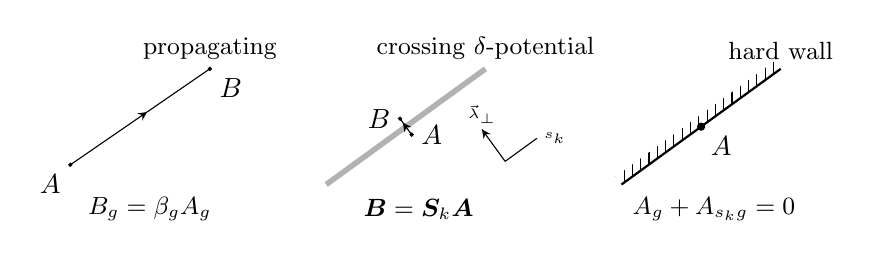
\begin{tikzpicture}[x=2.5cm, y=2.5cm]

\def\th{36}
\def\thth{36}
\def\shift{1.4}
\def\shiftshift{2.9}
\def\De{0.05}
\def\Dy{-0.125}
% 定义点
\coordinate (P1) at (0.1, 0.1);

\pgfmathsetmacro{\x}{cos(\th)}
\pgfmathsetmacro{\y}{sin(\th)}
\coordinate (P2) at (1.0*\x, 1.0*\y);

\pgfmathsetmacro{\x}{0.5*(0.1 + 0.8*cos(\th))}
\pgfmathsetmacro{\y}{\Dy}
\coordinate (P01) at (\x,\y);

\pgfmathsetmacro{\x}{\shift}
\pgfmathsetmacro{\y}{0}
\coordinate (P3) at (\x, \y);

\pgfmathsetmacro{\x}{cos(\thth)+\shift}
\pgfmathsetmacro{\y}{sin(\thth)}
\coordinate (P4) at (\x, \y);

\pgfmathsetmacro{\x}{cos(\thth)+\shift+0.1}
\pgfmathsetmacro{\y}{sin(\thth)*0.2}
\coordinate (PS0) at (\x, \y);

\pgfmathsetmacro{\x}{cos(\thth)+\shift+0.1 + 0.2*cos(\thth + 90)}
\pgfmathsetmacro{\y}{sin(\thth)*0.2 + 0.2*sin(\thth + 90)}
\coordinate (PS2) at (\x, \y);

\pgfmathsetmacro{\x}{cos(\thth)+\shift+0.1 + 0.2*cos(\thth)}
\pgfmathsetmacro{\y}{sin(\thth)*0.2 + 0.2*sin(\thth)}
\coordinate (PS1) at (\x, \y);

\pgfmathsetmacro{\x}{cos(\thth)/2-\De*cos(\thth+90)+\shift}
\pgfmathsetmacro{\y}{sin(\thth)/2-\De*sin(\thth+90)}
\coordinate (P5) at (\x, \y);

\pgfmathsetmacro{\x}{cos(\thth)/2+\De*cos(\thth+90)+\shift}
\pgfmathsetmacro{\y}{sin(\thth)/2+\De*sin(\thth+90)}
\coordinate (P6) at (\x, \y);

\pgfmathsetmacro{\x}{0.5*(0.0 + 1.0*cos(\thth)) + \shift}
\pgfmathsetmacro{\y}{\Dy}
\coordinate (P02) at (\x,\y);

\pgfmathsetmacro{\x}{\shiftshift}
\pgfmathsetmacro{\y}{0}
\coordinate (P7) at (\x, \y);

\pgfmathsetmacro{\x}{cos(\thth)+\shiftshift}
\pgfmathsetmacro{\y}{sin(\thth)}
\coordinate (P8) at (\x, \y);

\pgfmathsetmacro{\x}{cos(\thth)+\De*cos(\thth+90)+\shiftshift}
\pgfmathsetmacro{\y}{sin(\thth)+\De*sin(\thth+90)}
\coordinate (P9) at (\x, \y);

\pgfmathsetmacro{\x}{\De*cos(\thth+90)+\shiftshift}
\pgfmathsetmacro{\y}{\De*sin(\thth+90)}
\coordinate (P10) at (\x, \y);

\pgfmathsetmacro{\x}{cos(\thth)/2+\shiftshift}
\pgfmathsetmacro{\y}{sin(\thth)/2}
\coordinate (P11) at (\x, \y);

\pgfmathsetmacro{\x}{0.5*(0.0 + 1.0*cos(\thth)) + \shiftshift}
\pgfmathsetmacro{\y}{\Dy}
\coordinate (P03) at (\x,\y);

\node[mynode] at (P1) {};
\node[below left] at (P1) {$A$};
\node[mynode] at (P2) {};
\node[above] at (P2) {\small propagating};
\node[below right] at (P2) {$B$};
\draw[postaction={decorate}, 
      decoration={markings, mark=at position 0.55 with {\arrow{stealth}}}] (P1) -- (P2);

\draw[gray!60, line width=2.0] (P3) -- (P4);
\node[mynode] at (P5) {};
\node[above] at (P4) {\small crossing $\delta$-potential};
\node[right] at (P5) {$A$};
\node[mynode] at (P6) {};
\node[left] at (P6) {$B$};
\draw[postaction={decorate}, 
      decoration={markings, mark=at position 0.75 with {\arrow{stealth}}}] (P5) -- (P6);

\fill[pattern=vertical lines, pattern color=black] (P7) -- (P8) -- (P9) -- (P10) -- cycle;
\draw[black, thick] (P7) -- (P8);

\node[circle,        % 形状为圆形
        fill=black,    % 填充颜色为黑色
        inner sep=0.9, % 点的大小
        draw   ] at (P11) {};
\node[below right] at (P11) {$A$};
\node[above] at (P8) {\small hard wall};

\node[] at (P01) {\small $\quad \quad B_g=\beta_gA_g$};
\node[] at (P02) {\small $\quad \bm{B}=\bm{S}_k\bm{A}$};
\node[] at (P03) {\small \quad $A_g + A_{s_kg}=0$};

% \node[] at (PS0) {\tiny k};


\draw[postaction={decorate}] (PS0) -- (PS1);

      \draw[postaction={decorate}, 
      decoration={markings, mark=at position 1.00 with {\arrow{stealth}}}] (PS0) -- (PS2);
      
\node[above, yshift=-1.4pt] at (PS2) {\tiny $\vec{\lambda}_\perp$};
\node[right, xshift=-1pt] at (PS1) {\tiny $s_k$};

 
\end{tikzpicture}




\end{document}